\chapter{Implementation}
\label{cha:implementation}

This chapter will describe in detail the technical implementation of the Omni platform.

\section{Database}
\label{sec:impl-database}
Figure \ref{fig:db-erd} shows the final design of the tables. The Omni platform has two main entities that are easy to see, and a third arises during the implementation.

\begin{figure}[htbp]
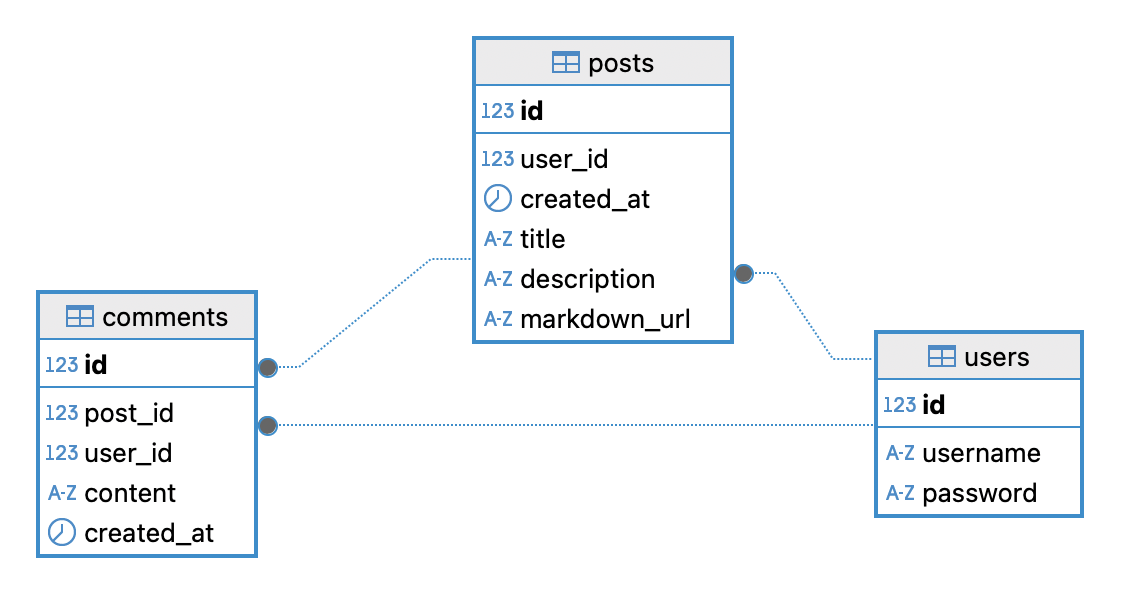
\includegraphics[width=12cm]{db-erd.png}
\centering
\caption{Database Entity Relationship Diagram}
\label{fig:db-erd}
\end{figure}

Information about each user needs to be stored, so a user table is naturally required. This includes any information about the user, such as username and password hash.
In the MVP of Omni, there is not much additional information stored about each user, but we could feasibly expand to store much more data for new features, such as storing a user's birthday.
In the future, if a hybrid approach for database distribution is used, a separate table to hold authentication data may be better to store this on a replicated database cluster rather than a sharded one.

The second easy-to-see table holds information about each post. It must store the creator's ID, title, description, link to the markdown file, timestamp, and more.
Posts will have a one-to-many relationship with users, where one user may create many posts, but each post is always associated with just one user. 

The final table is not as obvious to spot but still crucial: a table to store comments in. Storing this in the posts table does not make sense in a structured SQL database.
Adopting this approach could work in a NoSQL setup, but for popular posts, the document size would grow too big and slow down reading the post for everybody.
By storing the comments in a separate table, we can use pagination in our SQL queries to limit the number of comments we return to a user simultaneously.
This limits the load on the microservices, ensuring they are not overwhelmed by a very popular post with many comments.


